% the upright pyramid, cut open: Parts II and III keep its curvature at the apex, Parts IV and V spread it over the faces
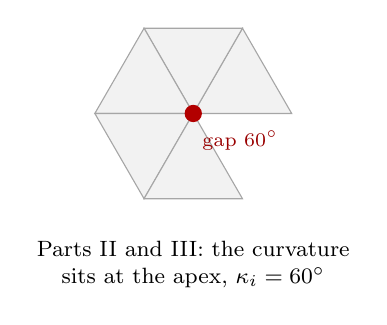
\begin{tikzpicture}[scale=1.25]
  \foreach \k in {0,...,4} {\filldraw[draw=gray!70, fill=gray!10] (0,0) -- ({60*\k}:1) -- ({60*(\k+1)}:1) -- cycle;}
  \fill[red!70!black] (0,0) circle (2.5pt);
  \node[red!60!black, font=\scriptsize] at (330:0.55) {gap $60^\circ$};
  \node[below, font=\footnotesize, align=center] at (0,-1.2) {Parts~II and~III: the curvature\\sits at the apex, $\kappa_i = 60^\circ$};
\end{tikzpicture}\hspace{1.5cm}
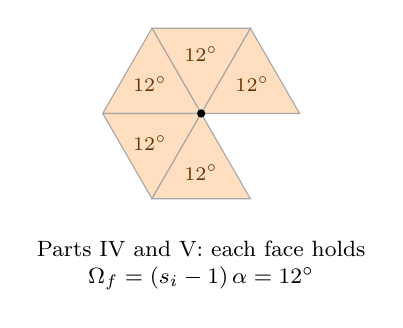
\begin{tikzpicture}[scale=1.25]
  \foreach \k in {0,...,4} {\filldraw[draw=gray!70, fill=orange!25] (0,0) -- ({60*\k}:1) -- ({60*(\k+1)}:1) -- cycle;
    \node[font=\scriptsize, orange!40!black] at ({60*\k+30}:0.6) {$12^\circ$};}
  \fill (0,0) circle (1.2pt);
  \node[below, font=\footnotesize, align=center] at (0,-1.2) {Parts~IV and~V: each face holds\\$\Omega_f = (s_i - 1)\,\alpha = 12^\circ$};
\end{tikzpicture}
